\bexo
Tracer sur la même figure
\begin{itemize}
	\item $t\mapsto \sin(t)$
	\item $t\mapsto 3\sin(-3t)$
	\item $t\mapsto -2\cos(2x)$ avec $x=\dfrac{\pi}{4}$
\end{itemize}
	
	\begin{center}
	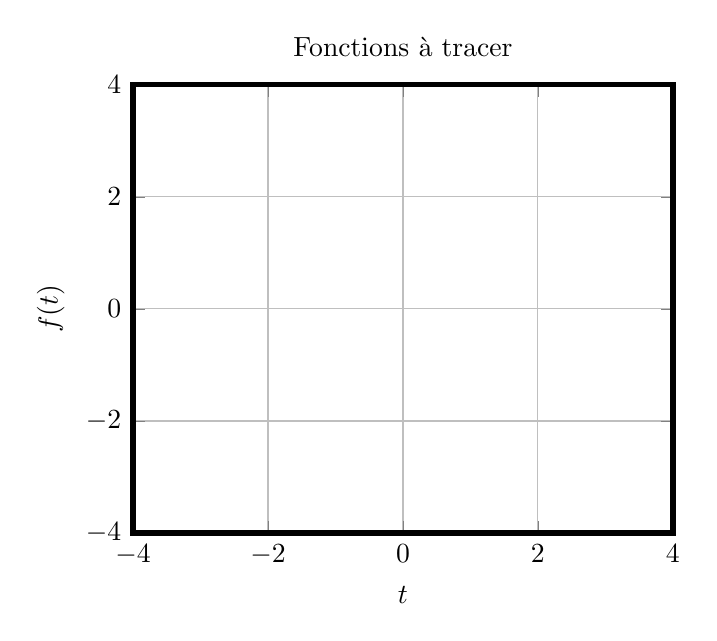
\begin{tikzpicture}
	  \begin{axis}[line width=2pt,       legend columns=-1,
   title=Fonctions à tracer,
   xlabel={$t$},
   ylabel={$f(t)$}, xmin=-4,
xmax=4,
ymin=-4, 
ymax=4,
	  legend to name=named , grid=major]
	%	\addplot[white] expression[domain=-pi:pi,samples=500]{4*cos(180*x/pi)};
				
	  \end{axis}

	\end{tikzpicture}
		  \ref{named}
\end{center}

	
	
	

\eexo
\solution{
Les graphes des fonctions sont:\\

	\begin{center}
	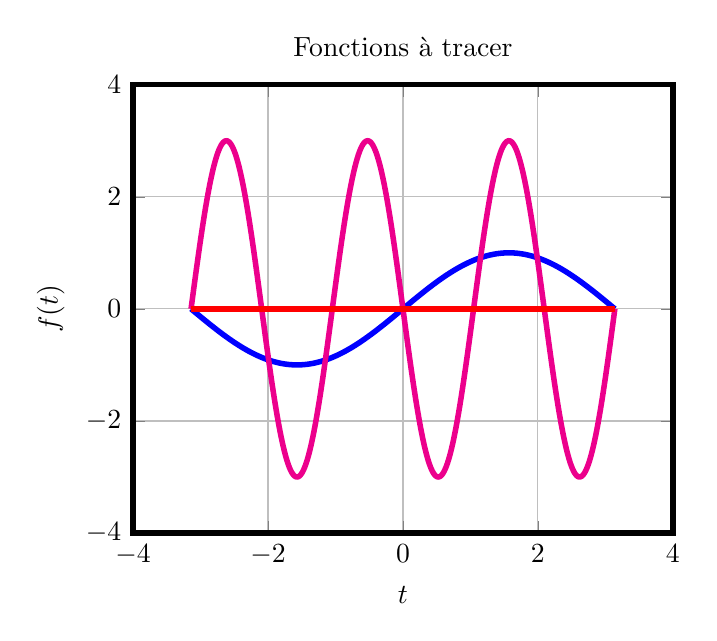
\begin{tikzpicture}
	  \begin{axis}[line width=2pt,       legend columns=-1,
   title=Fonctions à tracer,
   xlabel={$t$},
   ylabel={$f(t)$}, xmin=-4,
xmax=4,
ymin=-4, 
ymax=4,
legend entries={$\tr{sin}(t)$,$3\sin(-t)$,$-2\cos(2x)$},
	  legend to name=named , grid=major]
		\addplot[blue] expression[domain=-pi:pi,samples=500]{sin(180*x/pi)};
		\addplot[magenta,samples=500] expression[domain=-pi:pi]{-3*sin(3*180*x/pi)};
		\addplot[red,samples=500] expression[domain=-pi:pi]{0*cos(2*180*x/pi)};				  \end{axis}
	\end{tikzpicture}
		  \ref{named}
\end{center}


}